% Generated by pysimcount.pfchilds -- do not edit; regenerate instead.
% figure: main-cnot-suzuki-orders -- Suzuki formulas of each order, cnot gates vs n (layout of Childs et al. 2018 Fig. 3 right)
% source: ../np-main/aggregate.json + ../np-main-n9/seed{seed}, ../np-main-n11/seed{seed} (seeds [1, 2, 3, 4, 5, 6, 7, 8, 9, 10]); run commits: 01d3c275ceae2840002bd1aaea68f59b987c4975, e42ff29056ad9ea7fc7c9899fab334903e42e3e3
% metric=cnot kind=xyz merged (cz, simcount template)
% measured n: mean over seeds of the run's totals; bars min..max over seeds
% r from per-seed power-law fits (n = 5--11), mean count over seeds; r = ceil(a n^b); point=seed-mean; bars = min..max of per-seed fits
% per-step counts exactly affine in n (checked on n = [10, 20, 40], direct build at n = [100])
% shown: suzuki4, suzuki6, suzuki8
% removed (see main-cnot-suzuki-orders-ranking.md): lie-trotter, suzuki2
% figure made at git_commit=e5d9ee696f892e28aced765585653760f8a427c4 git_dirty=True
% WARNING: made from uncommitted code; the commit above does not reproduce it.
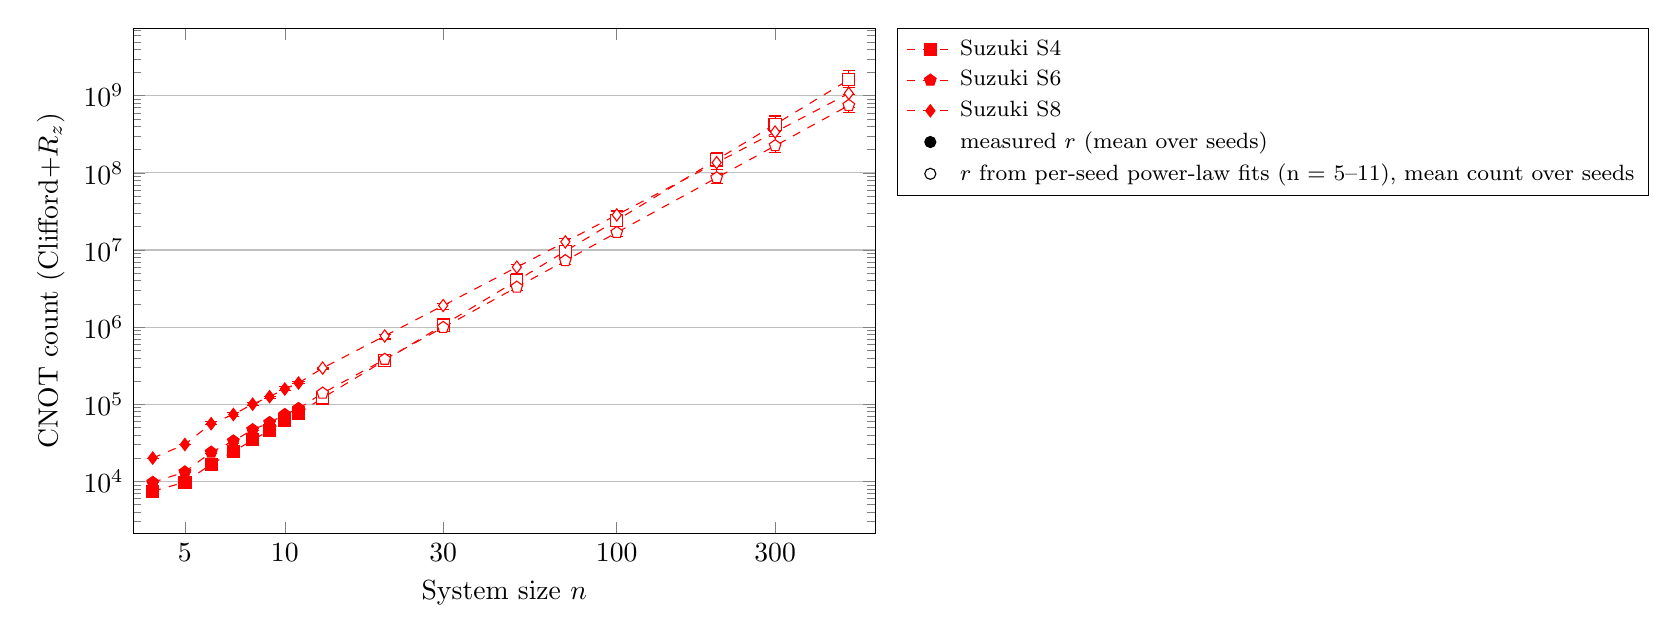
\begin{tikzpicture}
  \begin{loglogaxis}[
    width=11cm, height=8cm,
    xlabel={System size $n$},
    ylabel={CNOT count (Clifford+$R_z$)},
    xtick={5,10,30,100,300}, xticklabels={5,10,30,100,300},
    xmin=3.5, xmax=600,
    ymajorgrids=true,
    legend pos=outer north east,
    legend cell align=left,
    legend style={font=\footnotesize},
  ]
    % suzuki4: measured n, mean over seeds, bars min..max over seeds
    \addplot[red, dashed, mark=square*, mark size=2.2pt, mark options={solid, fill=red}, error bars/.cd, y dir=both, y explicit, error bar style={solid}] coordinates {
      (4,7459.2) += (0,100.8) -= (0,67.2)
      (5,9744) += (0,336) -= (0,294)
      (6,16707.6) += (0,1184.4) -= (0,831.6)
      (7,24284.4) += (0,1881.6) -= (0,1646.4)
      (8,34540.8) += (0,1411.2) -= (0,1276.8)
      (9,45549) += (0,2079) -= (0,2457)
      (10,62412) += (0,4788) -= (0,2352)
      (11,76230) += (0,3234) -= (0,1848)
    };
    \addlegendentry{Suzuki S4}
    % suzuki4: extrapolated, r = ceil(3.65267 n^1.59931), per step = 42 n + 0; bars min..max of per-seed fits
    \addplot[red, dashed, mark=square*, mark size=2.2pt, mark options={solid, fill=white}, mark indices={2,...,10}, forget plot, error bars/.cd, y dir=both, y explicit, error bar style={solid}] coordinates {
      (11,76230)
      (13,120830) += (0,5296.2) -= (0,3985.8)
      (20,370020) += (0,27300) -= (0,20580)
      (30,1.06155e+06) += (0,108990) -= (0,81270)
      (50,4.00848e+06) += (0,567420) -= (0,411180)
      (70,9.61968e+06) += (0,1.61112e+06) -= (0,1.14954e+06)
      (100,2.43394e+07) += (0,4.75398e+06) -= (0,3.34362e+06)
      (200,1.47922e+08) += (0,3.70709e+07) -= (0,2.53495e+07)
      (300,4.25239e+08) += (0,1.20644e+08) -= (0,8.11705e+07)
      (500,1.60899e+09) += (0,5.24758e+08) -= (0,3.46154e+08)
    };
    % suzuki6: measured n, mean over seeds, bars min..max over seeds
    \addplot[red, dashed, mark=pentagon*, mark size=2.2pt, mark options={solid, fill=red}, error bars/.cd, y dir=both, y explicit, error bar style={solid}] coordinates {
      (4,9696) += (0,0) -= (0,0)
      (5,13231) += (0,909) -= (0,101)
      (6,23876.4) += (0,1575.6) -= (0,848.4)
      (7,33370.4) += (0,1979.6) -= (0,2262.4)
      (8,46702.4) += (0,1777.6) -= (0,1454.4)
      (9,57812.4) += (0,2181.6) -= (0,3272.4)
      (10,73528) += (0,5252) -= (0,2828)
      (11,87991.2) += (0,3110.8) -= (0,1333.2)
    };
    \addlegendentry{Suzuki S6}
    % suzuki6: extrapolated, r = ceil(1.63295 n^1.35284), per step = 202 n + 0; bars min..max of per-seed fits
    \addplot[red, dashed, mark=pentagon*, mark size=2.2pt, mark options={solid, fill=white}, mark indices={2,...,10}, forget plot, error bars/.cd, y dir=both, y explicit, error bar style={solid}] coordinates {
      (11,87991.2)
      (13,139178) += (0,7878) -= (0,2626)
      (20,381780) += (0,30300) -= (0,14140)
      (30,989598) += (0,113322) -= (0,56358)
      (50,3.2926e+06) += (0,525200) -= (0,282800)
      (70,7.26796e+06) += (0,1.37158e+06) -= (0,749420)
      (100,1.68428e+07) += (0,3.70064e+06) -= (0,2.03616e+06)
      (200,8.62823e+07) += (0,2.43733e+07) -= (0,1.34411e+07)
      (300,2.24481e+08) += (0,7.17928e+07) -= (0,3.94688e+07)
      (500,7.49087e+08) += (0,2.75659e+08) -= (0,1.50258e+08)
    };
    % suzuki8: measured n, mean over seeds, bars min..max over seeds
    \addplot[red, dashed, mark=diamond*, mark size=2.2pt, mark options={solid, fill=red}, error bars/.cd, y dir=both, y explicit, error bar style={solid}] coordinates {
      (4,20040) += (0,0) -= (0,0)
      (5,30060) += (0,0) -= (0,0)
      (6,55911.6) += (0,4208.4) -= (0,1803.6)
      (7,73647) += (0,3507) -= (0,3507)
      (8,100200) += (0,4008) -= (0,4008)
      (9,125350) += (0,901.8) -= (0,8116.2)
      (10,157314) += (0,13026) -= (0,7014)
      (11,188476) += (0,9919.8) -= (0,1102.2)
    };
    \addlegendentry{Suzuki S8}
    % suzuki8: extrapolated, r = ceil(0.896539 n^1.24879), per step = 1002 n + 0; bars min..max of per-seed fits
    \addplot[red, dashed, mark=diamond*, mark size=2.2pt, mark options={solid, fill=white}, mark indices={2,...,10}, forget plot, error bars/.cd, y dir=both, y explicit, error bar style={solid}] coordinates {
      (11,188476)
      (13,294388) += (0,5210.4) -= (0,7815.6)
      (20,767532) += (0,34068) -= (0,66132)
      (30,1.9028e+06) += (0,141282) -= (0,219438)
      (50,5.99196e+06) += (0,571140) -= (0,981960)
      (70,1.27444e+07) += (0,1.42384e+06) -= (0,2.36372e+06)
      (100,2.84768e+07) += (0,3.58716e+06) -= (0,6.13224e+06)
      (200,1.35591e+08) += (0,2.13226e+07) -= (0,3.63926e+07)
      (300,3.38205e+08) += (0,5.94887e+07) -= (0,1.01032e+08)
      (500,1.07024e+09) += (0,2.13326e+08) -= (0,3.57814e+08)
    };
    \addlegendimage{only marks, black, mark=*, mark options={solid, fill=black}}
    \addlegendentry{measured $r$ (mean over seeds)}
    \addlegendimage{only marks, black, mark=*, mark options={solid, fill=white}}
    \addlegendentry{$r$ from per-seed power-law fits (n = 5--11), mean count over seeds}
  \end{loglogaxis}
\end{tikzpicture}
